\section{\filetotitle}
In this section, we will explore the concept of coherence in mixed quantum-classical dynamics and how well it can be described by \acrshort{tsh}. First, we will introduce the concept of coherence and its importance in quantum mechanics. Then, we will discuss how \acrshort{tsh} can capture coherence effects in mixed quantum-classical systems. Finally, we will present some examples and results to illustrate the effectiveness of \acrshort{tsh} in describing coherence in these systems.
\subsection{Coherence in Trajectory Surface Hopping}\label{sec:coherence_in_sh}
While mixed quantum-classical dynamics methods are routinely used to simulate nonadiabatic population transfer, accurately predicting the quantum phase and therefore the coherence between electronic states remains a significant challenge. Coherence is a fundamental aspect of quantum mechanics that describes the phase relationship between different quantum states.

In standard density matrix formalism, the diagonal elements $\rho_{II}$ represent the population of state $I$, while the off-diagonal elements $\rho_{IJ}$ (for $I\neq J$) represent the coherence between states $I$ and $J$. In a fully quantum mechanical treatment, both populations and coherences evolve according to the \acrshort{tdse}. Since two out of three \acrshort{tsh} methods (\acrshort{lzsh} and \acrshort{mash}) were derived for two-state systems, we will focus our efforts on analyzing the coherence between two states. For two-state systems it is highly convenient to represent the density matrix in the form of a Bloch vector $\symbf{\sigma}=(s_x,s_y,s_z)$, where
\begin{equation}
\sigma_x=2\Re\rho_{01},\quad\sigma_y=2\Im\rho_{01},\quad\sigma_z=\rho_{11}-\rho_{00}.
\end{equation}
Besides the bloch vector $\symbf{\sigma}$, we will also define the quantity $\sigma_\perp=\sqrt{\sigma_x^2+\sigma_y^2}$, which represents the magnitude of the coherence between the two states. In a fully quantum mechanical treatment, the coherence $\sigma_\perp$ can range from 0 (completely incoherent) to 1 (fully coherent). In \acrshort{tsh} methods, the coherence is often underestimated due to the classical treatment of nuclear motion and the stochastic nature of surface hopping.

To understand why capturing coherence is critical, consider a potential with two electronic states and two consecutive avoided crossings. Let the system be initially prepared in the upper state. Before the first avoided crossing, the system is fully coherent, with $\sigma_\perp=1$. If the system never encounters the second avoided crossing, the final populations ale determined purely by the transition probability at the first avoided crossing. In this single-crossing scenario, the subsequent decay or mishandling of the coherence magnitude $\sigma_\perp$ does not affect the final populations.

However, handling of the relative phase between the two states, which is directly related to the coherence, becomes crucial when the system encounters the second avoided crossing. Between the first crossing at a time $t_1$ and the second crossing at a time $t_2$, the system evolves as a superposition of the two states and the components of the wavepacket propagate on their respective adiabatic surfaces $E_0(\symbf{R}(t))$ and $E_1(\symbf{R}(t))$. During this time interval, they accumulate a relative phase
\begin{equation}
\Delta\Phi=\Phi_1-\Phi_0=\int_{t_1}^{t_2}E_1(\symbf{R}(t))\dt-\int_{t_1}^{t_2}E_0(\symbf{R}(t))\dt=\int_{t_1}^{t_2}\Delta E(\symbf{R}(t))\dt,
\end{equation}
where $\Phi_0$ and $\Phi_1$ are the phases accumulated by the components of the wavepacket on the lower and upper surfaces, respectively, and $\Delta E(\symbf{R}(t))=E_1(\symbf{R}(t))-E_0(\symbf{R}(t))$ is the energy gap between the two surfaces. When the branches of the wavepacket encounter the second avoided crossing, the transition probability at this crossing depends on the relative phase $\Delta\Phi$. The amplitudes arriving at the second crossing are therefore $\tilde c_0=c_0e^{i\Phi_0}$ and $\tilde c_1=c_1e^{i\Phi_1}$, where $c_0$ and $c_1$ are the amplitudes of the wavepacket components on the lower and upper surfaces, respectively, at the time of the second crossing. Note that while the phase of $\rho_{01}$ oscillates in between the two crossings, the magnitude $\sigma_\perp$ remains constant.

When the system encounters the second avoided crossing, the states mix again, which can be described by a unitary evolution operator $U$ of the amplitudes $\tilde c_0$ and $\tilde c_1$ as
\begin{align}
c_0^{\symrm{final}}&=U_{00}\tilde c_0+U_{01}\tilde c_1,\\
c_1^{\symrm{final}}&=U_{10}\tilde c_0+U_{11}\tilde c_1,
\end{align}
where $U_{00}$, $U_{01}$, $U_{10}$, and $U_{11}$ are the elements of the unitary operator $U$ in the basis of adiabatic states and $\c_0^{\symrm{final}}$ and $\c_1^{\symrm{final}}$ are the final amplitudes after the second crossing. The final population of, let's say, the upper state is then given by $\rho_{11}^{\symrm{final}}=|c_1^{\symrm{final}}|^2$, which can be expanded as
\begin{equation}
\rho_{11}^{\symrm{final}}=|U_{10}|^2|\tilde c_0|^2+|U_{11}|^2|\tilde c_1|^2+2\Re\left(U_{10}^*U_{11}\tilde c_0^\ast\tilde c_1\right).
\end{equation}
The first two terms in the expression above represent classical, incoherent contributions to the final population. This is what standard surface hopping methods capture. The last term, however, represents a quantum interference contribution to the final population, which depends on the relative phase $\Delta\Phi$ and the coherence magnitude $\sigma_\perp$. This interference term can lead to constructive or destructive interference, significantly affecting the final population distribution. Therefore, accurately capturing both the magnitude and phase of the coherence is essential for correctly predicting the outcomes of nonadiabatic dynamics in systems with multiple avoided crossings.
\subsection{The Landau--Zener Scattering Matrix}
Now that we have established the importance of coherence in nonadiabatic dynamics, we can analyze how well \acrshort{tsh} methods capture this coherence. We already know how to extract coherences from the \acrshort{mash}, since it is based on propagating directly the Bloch vector $\symbf{\sigma}$. For \acrshort{fssh} it is also straightforward to extract the coherence, since it is based on propagating the electronic coefficients $c_I$. For \acrshort{lzsh}, however, the situation is not as straightforward, since it does not propagate anything during the dynamics.

To extract the coherence from \acrshort{lzsh}, we must extend its standard formalism. As derived in Section~\ref{sec:landau_zener}, the traditional Landau--Zener formula provides the asymptotic transition probability $P=\e^{-2\pi\Gamma}$, where $\Gamma=\frac{g^2}{4\alpha}$ (see Section~\ref{sec:landau_zener}). However, this formula is merely a squared modulus of the off-diagonal element of the scattering matrix $S$ that describes the transition between the two states. By utilizing only $P$, the \acrshort{lzsh} method effectively discards the phase information contained in the scattering matrix, which is crucial for describing coherence. The $S$ matrix is a mathematical operator that maps tthe asymptotic incoming wavepacket amplitudes to the asymptotic outgoing wavepacket amplitudes after passing through the crossing as
\begin{equation}
\begin{pmatrix}
c_0(t\to+\infty)\\
c_1(t\to+\infty)
\end{pmatrix}=S\begin{pmatrix}
c_0(t\to-\infty)\\
c_1(t\to-\infty)
\end{pmatrix}.
\end{equation}
This holds for any representation we choose. In the adiabatic representation, the unitary scattering matrix $S$ can be expressed, without derivation, as
\begin{equation}
S=\begin{pmatrix}
\sqrt{1-P}e^{-i\phi_S}&-\sqrt{P}\\
\sqrt{P}&\sqrt{1-P}e^{i\phi_S}
\end{pmatrix},
\end{equation}
where $\phi_S$ is the Stokes phase, which can be calculated as
\begin{equation}
\phi_S=\frac{\pi}{4}+\Gamma\left(\ln\Gamma-1\right)+\arg\Gamma_f(1-i\Gamma),
\end{equation}
where we were forced to denote the gamma function with a subscript $f$ as $\Gamma_f$ to avoid confusion with the $\Gamma$ parameter in the Landau--Zener formula. By utilizing the full scattering matrix $S$, we can extract both the transition probability and the phase information, allowing us to capture the coherence effects in \acrshort{lzsh}. Note that the Stokes phase $\phi_S$ only accounts for the phase shift during the crossing, but does not account for the phase accumulation during the propagation on the adiabatic surfaces. Therefore, subsequent crossings cannot be described by simply multiplying the scattering matrices of each crossing, since the relative phase between the states at the second crossing would not be correctly captured.

Part of the motivation for this section was to analyze how well \acrshort{lzsh} captures coherence effects. To do this, the implementation of \acrshort{lzsh} was extended to utilize the full scattering matrix $S$ instead of just the transition probability $P$. This allows us to extract the coherence from \acrshort{lzsh} and compare it against the exact quantum mechanical results. After implementing this extension, we applied it to the original \acrshort{lzsh} model in Eq~\eqref{eq:landau_zener_hamiltonian}, with parameters $g=4$~a.u. and $\alpha=20$~a.u. As shown in Figure~\ref{fig:lzsh_coherence_comparison}, the coherences obtained from the \acrshort{lzsh} scattering matrix are in perfect agreement with the exact quantum mechanical results, as expected since both results should be identical.
\begin{figure}[H]
\centering
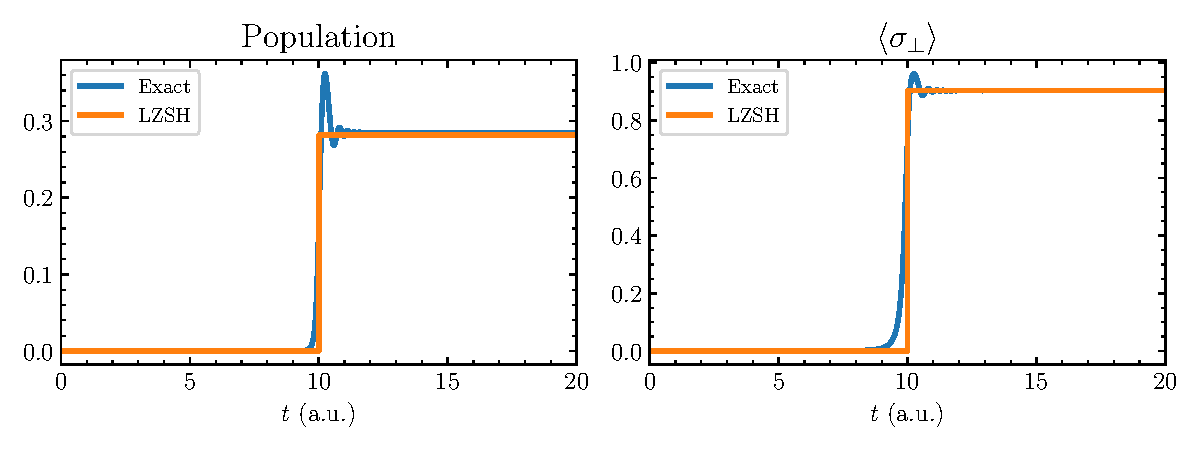
\includegraphics[width=\linewidth]{chapters/04-Supporting_Numerical_Studies/sections/images/LZSH_COMPARE}
\caption{Comparison of the coherences obtained from the \acrshort{lzsh} scattering matrix with the exact quantum mechanical results for the original \acrshort{lzsh} model (Eq.~\eqref{eq:landau_zener_hamiltonian}), where both results should be identical. The simulations were performed with parameters $g=4$~a.u. and $\alpha=20$~a.u. and 10000 trajectories.}
\label{fig:lzsh_coherence_comparison}
\end{figure}
These results confirm that the \acrshort{lzsh} method, along with the scattering matrix extension, is correctly implemented and we can move on to analyzing more complex models. The simulations in Fig.~\ref{fig:sh_coherence_comparison} also confirm correct implementation of all the components of nonadiabatic dynamics methods, since the populations match the exact result, as well as the correctness of the exact quantum mechanical results.
\subsection{Coherence in Avoided Crossing Dynamics}
To evaluate the performance of the \acrshort{lzsh}, \acrshort{fssh}, and \acrshort{mash} methods in capturing coherence effects, we applied them to a standard avoided crossing model with Hamiltonian
\begin{equation}
H^{\symrm{el}}=\begin{pmatrix}
\frac{1}{2}m\omega^2x^2+\kappa x+\epsilon&\delta\\
\delta&\frac{1}{2}m\omega^2x^2-\kappa x-\epsilon
\end{pmatrix},
\end{equation}
where $m=1$~a.u., $\omega=1$~a.u., $\kappa=3$~a.u., $\epsilon=4$~a.u., and $\delta=2$~a.u. The system was initialized in the upper state with a Gaussian nuclear wavepacket centered at $x=3$~a.u. with zero momentum. The simulations were performed with 100000 trajectories for each method. The simulations were set up this way so that the system encounters two consecutive avoided crossings, allowing us to analyze the importance of coherence effects in this scenario.

Fig.~\ref{fig:sh_coherence_comparison} presents the time evolution of the Bloch vector components $\sigma_x$, $\sigma_y$, and $\sigma_z$, as well as the coherence magnitude $\sigma_\perp$ obtained from the \acrshort{lzsh}, \acrshort{fssh}, and \acrshort{mash} methods, compared against the exact quantum mechanical results. The results show that all three methods capture the general trend of the population transfer between the two states, as indicated by the agreement in $\sigma_z$. However, there are significant differences in how well they capture the coherence effects.

\begin{figure}[H]
\centering
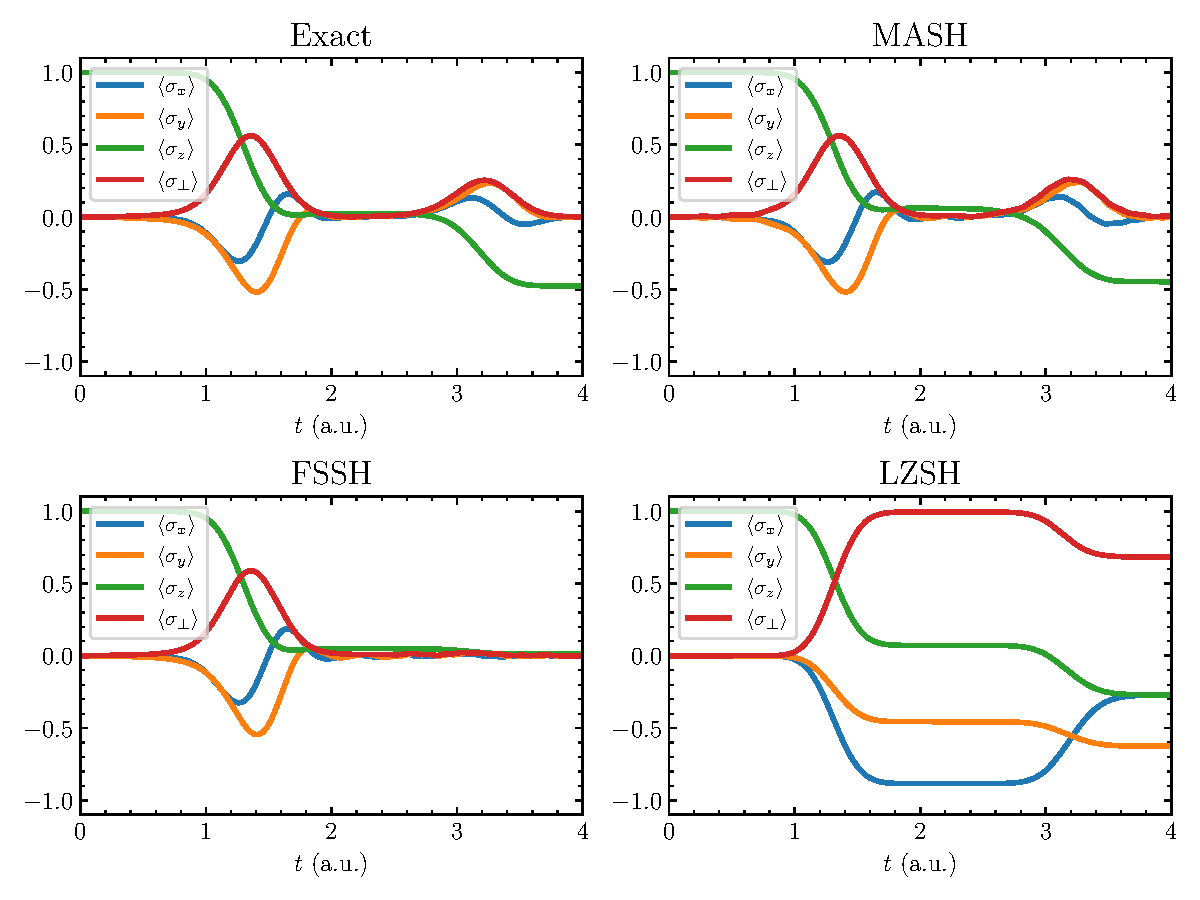
\includegraphics[width=\linewidth]{chapters/04-Supporting_Numerical_Studies/sections/images/SH_COHERENCE_COMPARE}
\caption{Comparison of the coherences obtained from the \acrshort{lzsh}, \acrshort{fssh}, and \acrshort{mash} against the exact quantum mechanical results for an avoided crossing model.}
\label{fig:sh_coherence_comparison}
\end{figure}

The \acrshort{mash} approach exhibits the best agreement with the exact quantum mechanical results for the coherence. This is not unexpected, since \acrshort{mash} is designed to propagate the full Bloch vector, allowing it to capture both the magnitude and phase of the coherence accurately. The \acrshort{fssh} method captures the coherences correctly up until the second avoided crossing, since the relative phase between the states is treated incorrectly after the first crossing. This is also a known issue with \acrshort{fssh}.

The novel approach in \acrshort{tsh}, the usage of scattering matrix $S$ during \acrshort{lzsh} dynamics, captures a general trend of the coherence, but it significantly overestimates the coherence magnitude $\sigma_\perp$ after the first crossing. This could be caused by the fact that the scattering matrix $S$ only accounts for the phase shift during the crossing, but does not account for the phase accumulation during the propagation on the adiabatic surfaces. For this reason, subsequent crossings cannot be described by simply multiplying the scattering matrices of each crossing, since the relative phase between the states at the second crossing would not be correctly captured.

Overall, capturing coherence effects in mixed quantum-classical dynamics is hardly a solved problem. While \acrshort{mash} performs well in this regard, it is not widely used due to its significantly different formalism and absence of a rigorous derivation for multi-state systems. The \acrshort{fssh} method, while widely used, has known issues with capturing coherence effects, especially in scenarios with multiple avoided crossings. The \acrshort{lzsh} method, even with the extension to utilize the full scattering matrix, still struggles to accurately capture coherence effects due to its inherent limitations in describing phase accumulation during propagation. Therefore, further research and development are needed to improve the ability of mixed quantum-classical dynamics methods to capture coherence effects accurately.
